\documentclass[a4paper,10pt]{article}
\usepackage[dvips]{graphicx}
\usepackage{fancybox}

\begin{document}

Differences between circular and triangular coils are related to the geometry of the coils, frequency response and radiation pattern. However, these differences produce similar results.

The difference in the geometry of the coils cause subtle changes in the inductance altering its resonant frequency. Figure \ref{fig:exp_1} was obtained by a \emph{S} parameters analizer and it show several resonant frequencies for tha circular and triangular coils. From this figure, the first resonant frequencies can be observed between 21 MHz and 26 MHz for both kind of coils. It's important to remember that two circular (or triangular) coils were used in all experimets in order to complete teh system Transmitter-Receiver.
%\vspace{3mm}

\begin{figure}[tbp]
\begin{center}
\fbox{
\begin{tabular}{cc}
\scalebox{0.35}[0.4]{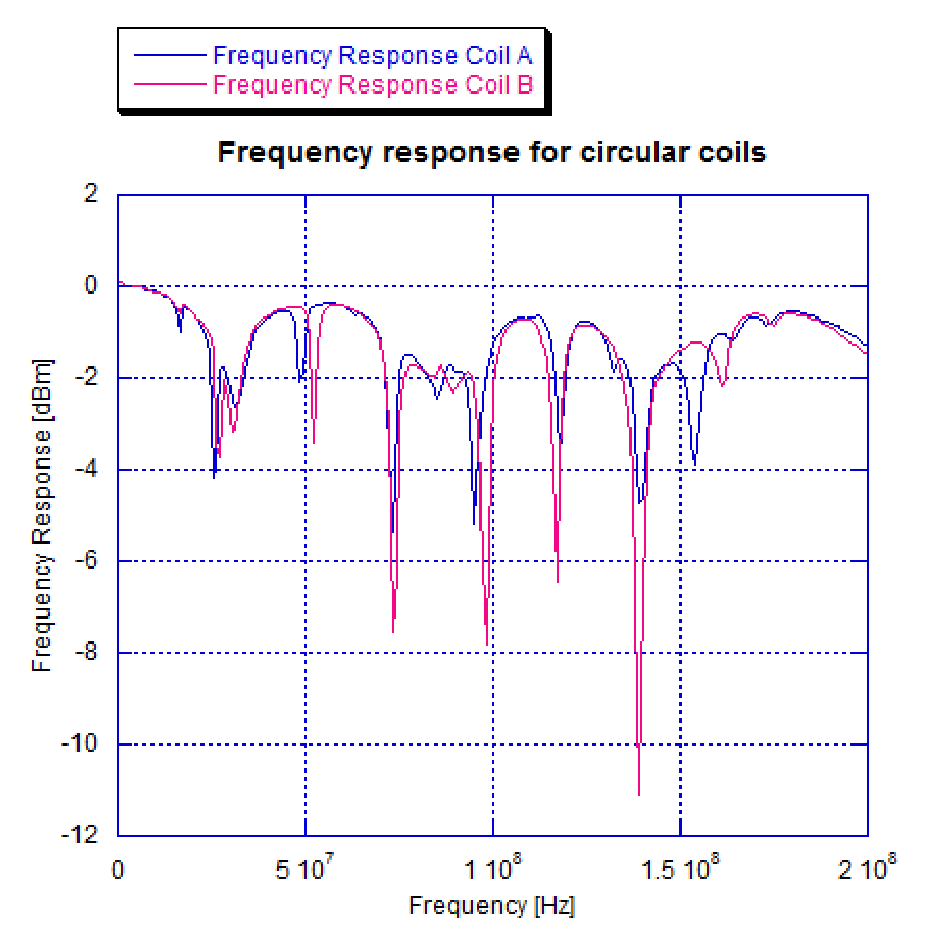
\includegraphics{01_circulares.eps}}&
\scalebox{0.35}[0.4]{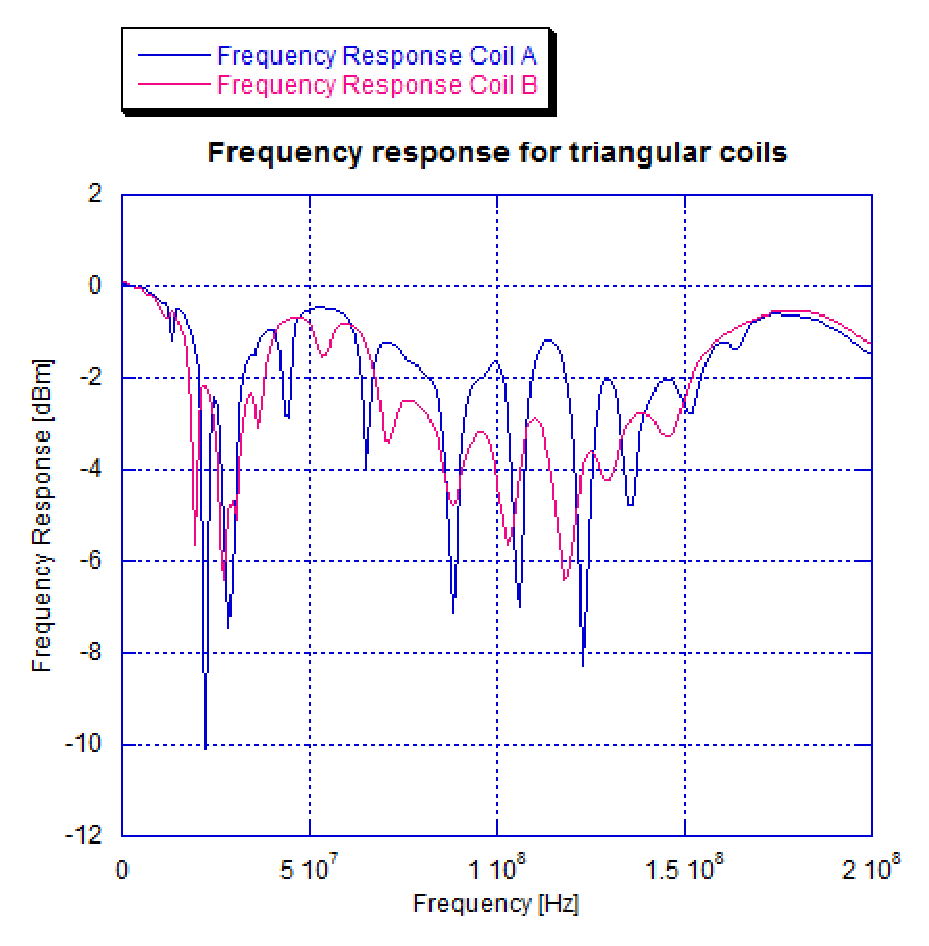
\includegraphics{02_triangulares.eps}}\\
a)&b)\\
\end{tabular}
} \caption{Resonant frequencies for the circular (a) coils and (b) triangular before 200 MHz.}\label{fig:exp_1}
\end{center}
\end{figure}

In order to define the working frequency, each pair of coils was tested with a RF generator and a spectrum analizer. Figure \ref{fig:exp_2} shows the frequency sweep for circular coils, in the same way, figure \ref{fig:exp_3} present the frequency sweep for triangular coils. The working frequency can be observed between 21 MHz and 27 MHz. This range of frequencies is due to the coils are not perfects and identical neither.

\begin{figure}[tbp]
\begin{center}
\fbox{
\begin{tabular}{cc}
\scalebox{0.3}[0.4]{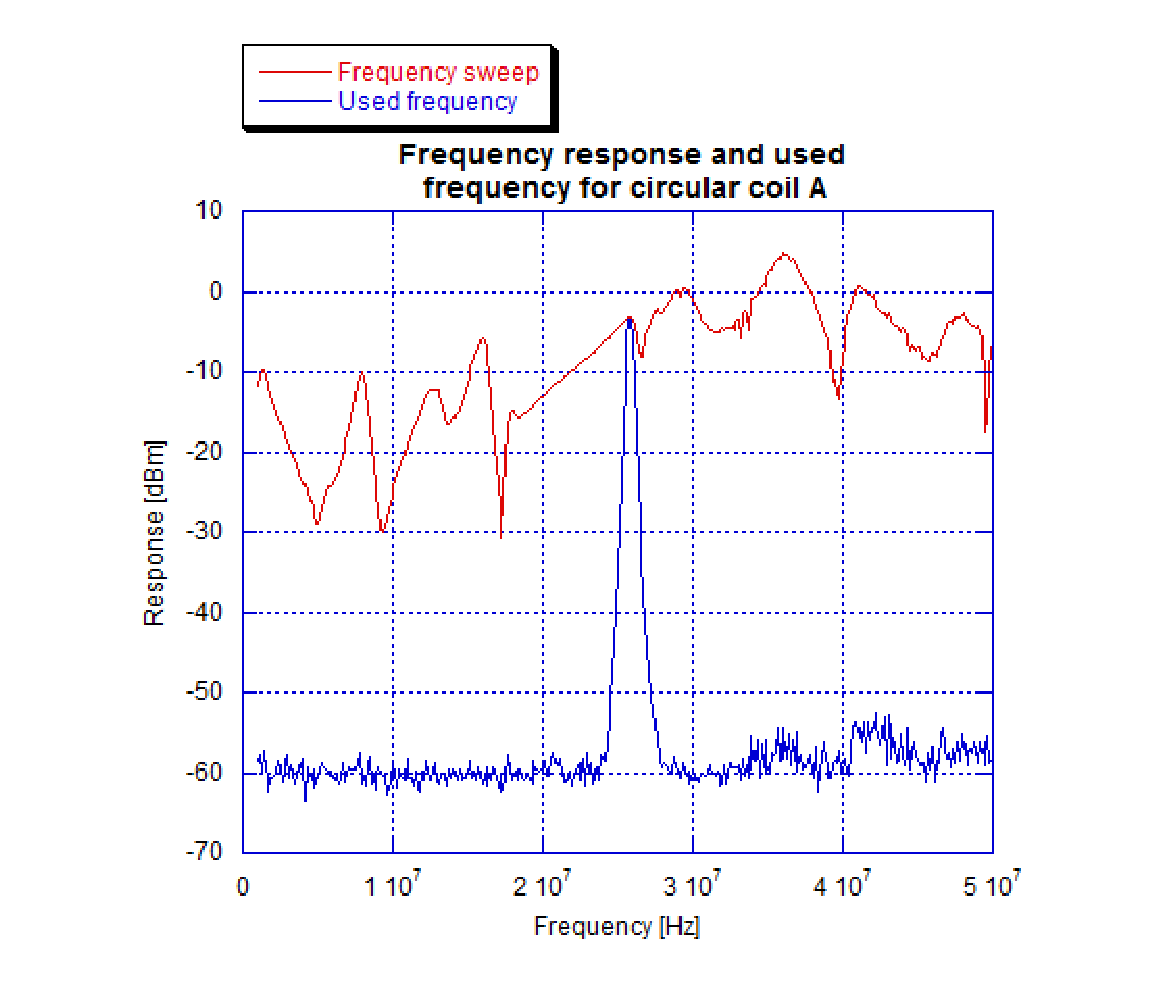
\includegraphics{03_distribucion_circular_A.eps}}&
\scalebox{0.3}[0.4]{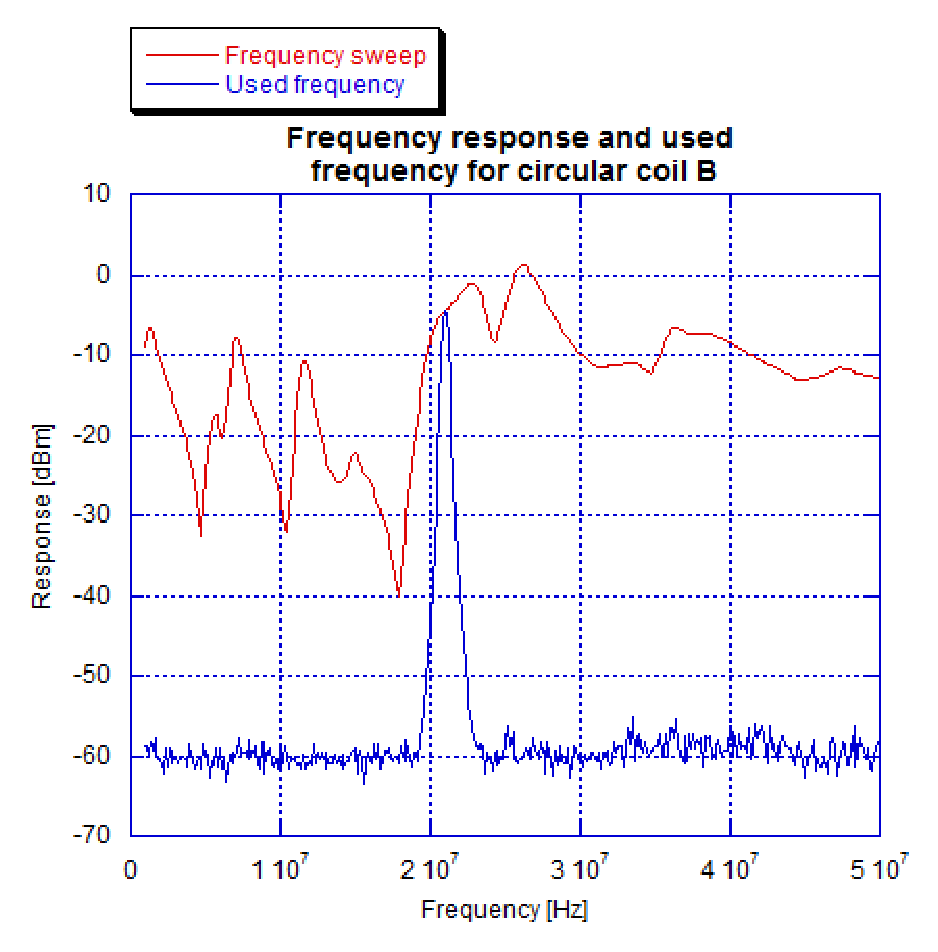
\includegraphics{04_distribucion_circular_B.eps}}\\
a)&b)\\
\end{tabular}
} \caption{Frequency sweep and working frequency for the pair of circular coils.}\label{fig:exp_2}
\end{center}
\end{figure}

\begin{figure}[tbp]
\begin{center}
\fbox{
\begin{tabular}{cc}
\scalebox{0.35}[0.4]{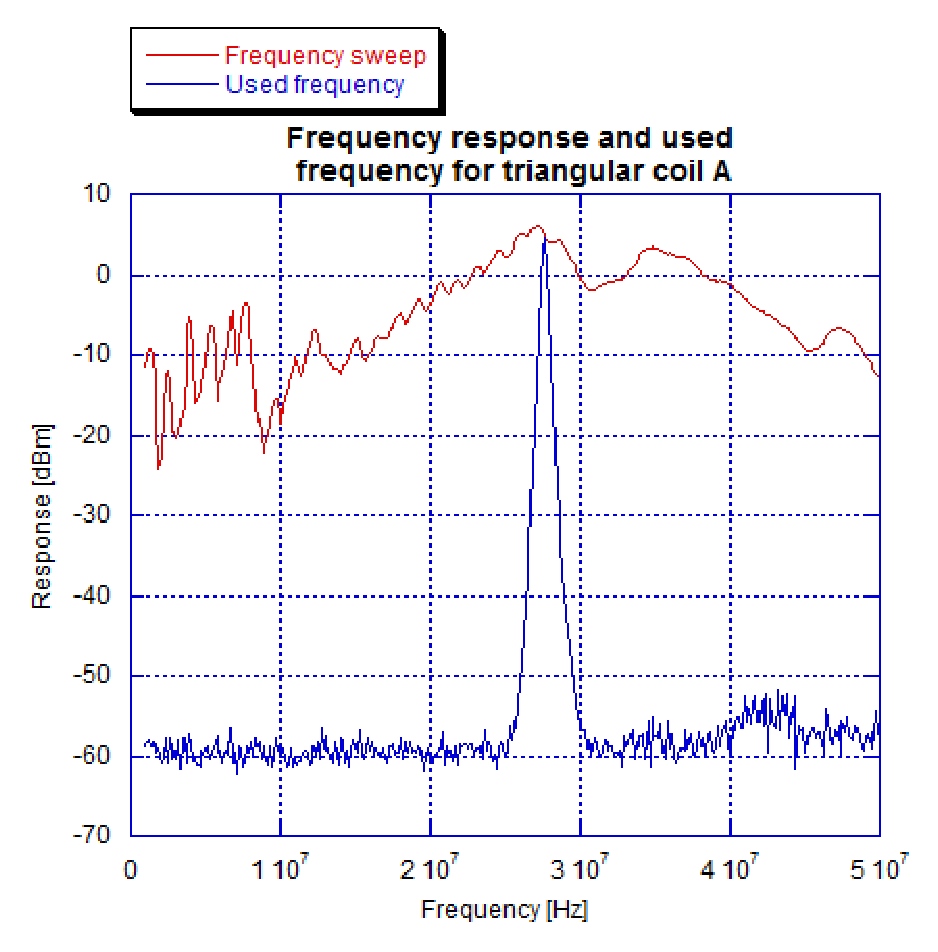
\includegraphics{05_distribucion_triangular_A.eps}}&
\scalebox{0.35}[0.4]{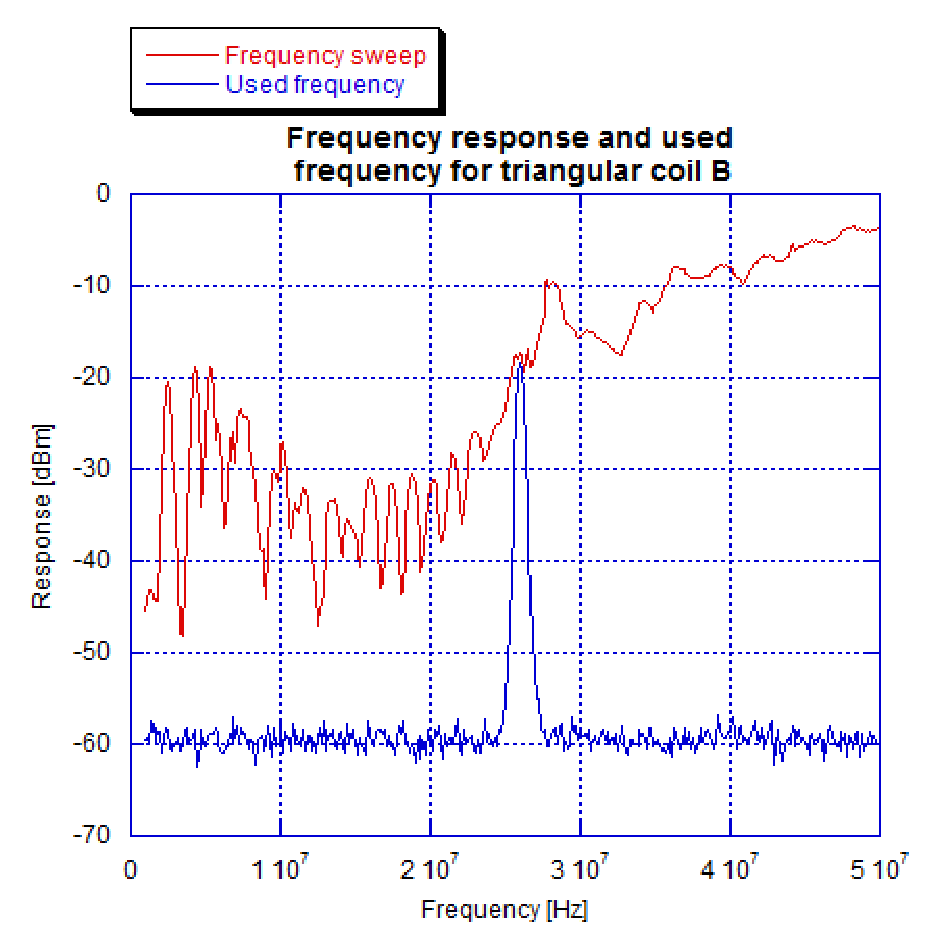
\includegraphics{06_distribucion_triangular_B.eps}}\\
a)&b)\\
\end{tabular}
} \caption{Frequency sweep and working frequency for the pair of triangular coils.}\label{fig:exp_3}
\end{center}
\end{figure}

Once the working frequencies were found for each pair of (circular and triangular) coils, the energy transfer experiment was completed. In this experiment, the RF generator was connected to one circular or triangular coil (called transmitter coil) and the spectrum analizer was conected to another circular or triangular coil (called receiver coil). Initially, both coils was separated 0 cm. After that, one coil was displaced to 25 cm in 1 cm steps. Figure \ref{fig:exp_4} shows the received power for circular and triangular coils in a range form 0 cm to 25 cm. The frequency distribution (for four distances) is shown in figure \ref{fig:exp_5}. In this figure it can be observed that the amplitude, the bandwidth and the spectral density decrease also.

\begin{figure}[tbp]
\begin{center}
\fbox{
\begin{tabular}{cc}
\scalebox{0.35}[0.4]{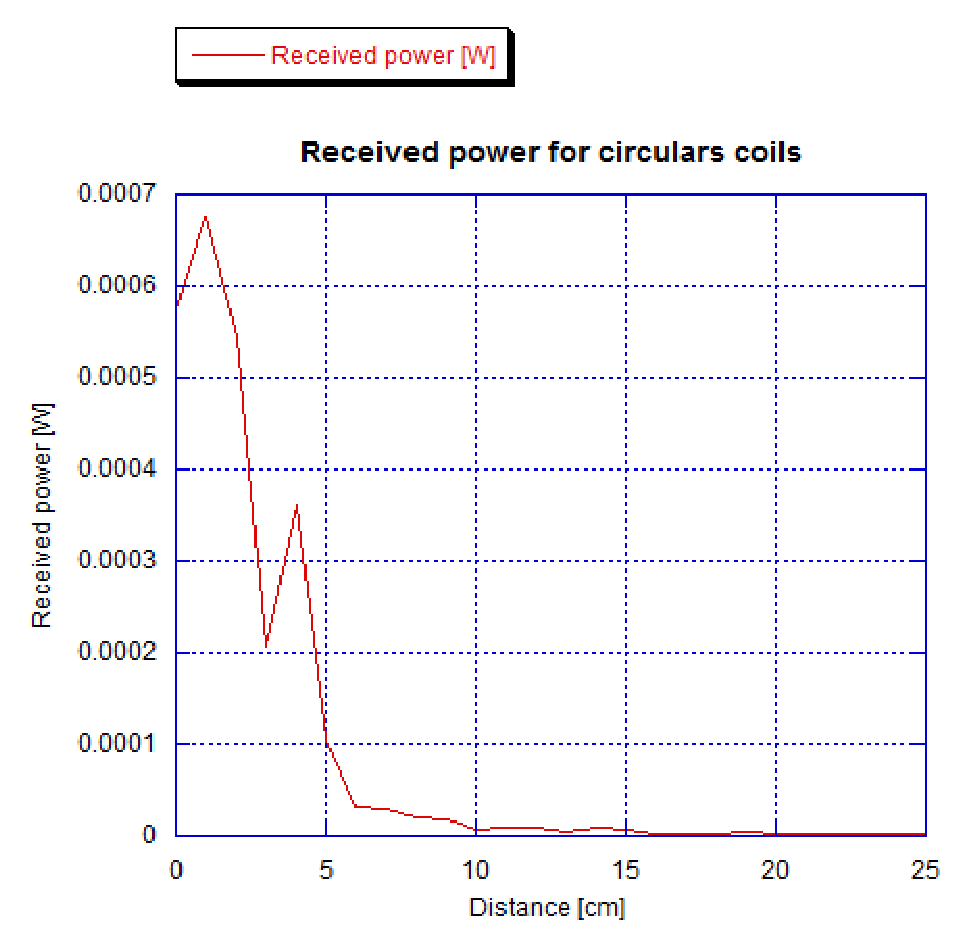
\includegraphics{09_reponse_circular.eps}}&
\scalebox{0.35}[0.4]{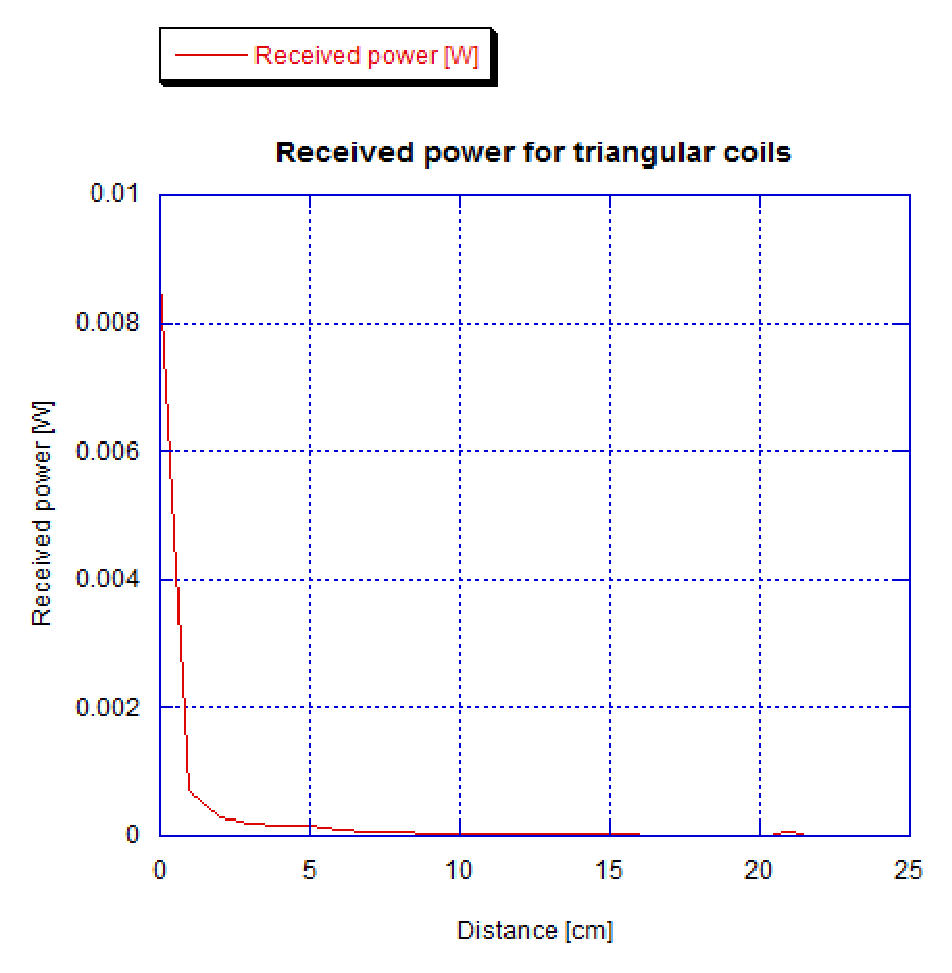
\includegraphics{10_reponse_triangular.eps}}\\
a)&b)\\
\end{tabular}
} \caption{Received power for (a) circular and (b) triangular coils.}\label{fig:exp_4}
\end{center}
\end{figure}

\begin{figure}[tbp]
\begin{center}
\fbox{
\begin{tabular}{cc}
\scalebox{0.35}[0.4]{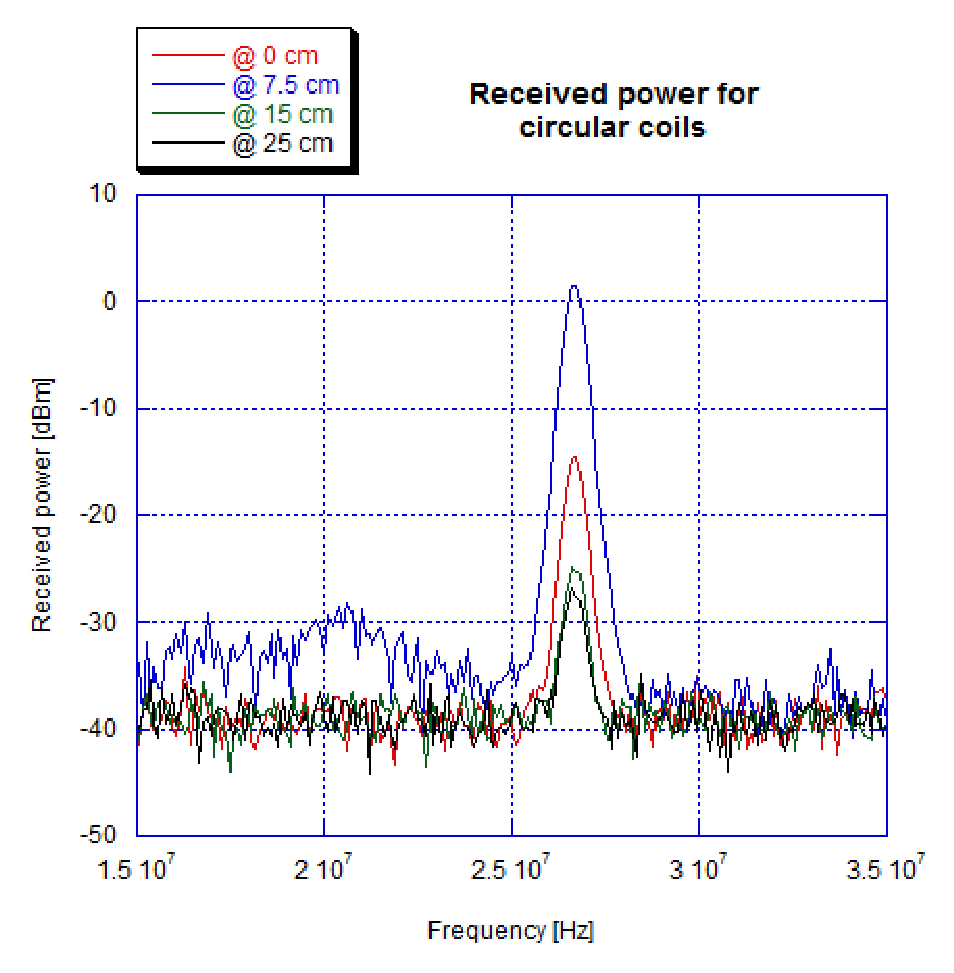
\includegraphics{07_received_power_circular.eps}}&
\scalebox{0.35}[0.4]{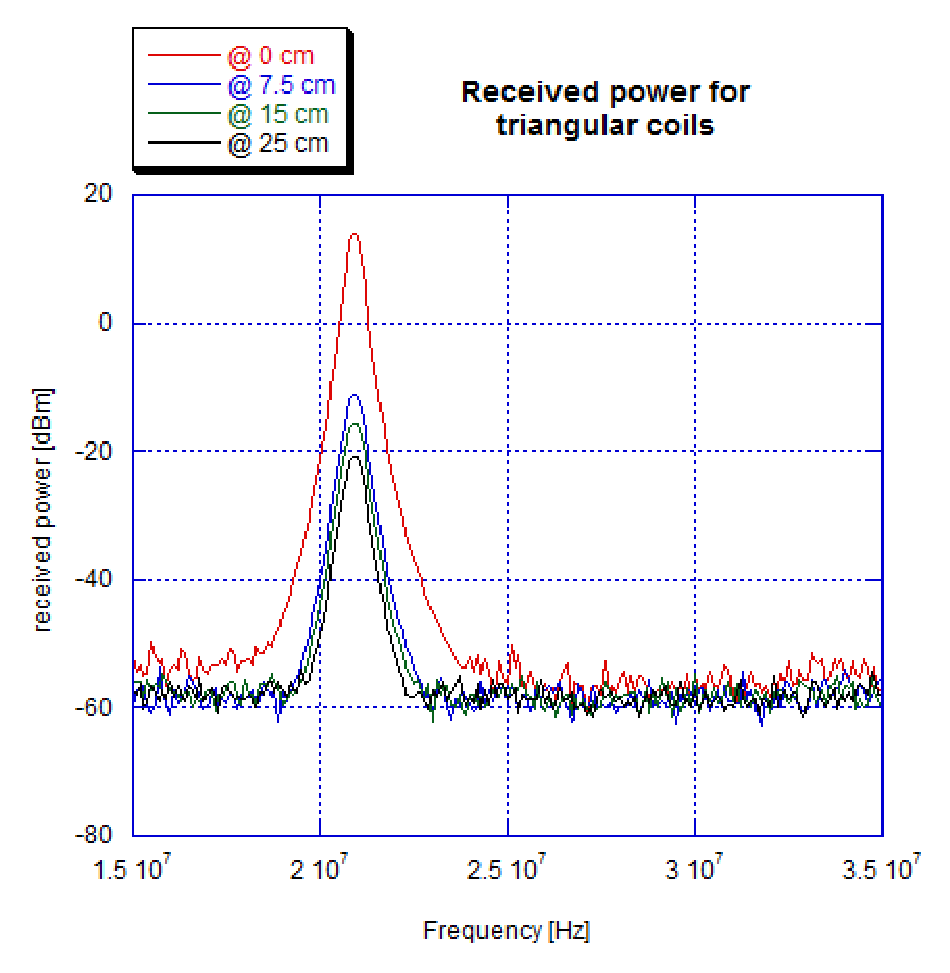
\includegraphics{08_received_power_triangular.eps}}\\
a)&b)\\
\end{tabular}
} \caption{Received power for 4 distances for (a) circular and (b) triangular coils.}\label{fig:exp_5}
\end{center}
\end{figure}

The normalized efficiency of the receiver coil was calculated considering that the maximum power will be always close of 0 cm. In this scheme, the efficiency is proportional to received power (see figure \ref{fig:exp_5}). Figure \ref{fig:exp_6} show the efficiency fo circular an triangular coils.

\begin{figure}[tbp]
\begin{center}
\fbox{
\begin{tabular}{cc}
\scalebox{0.35}[0.4]{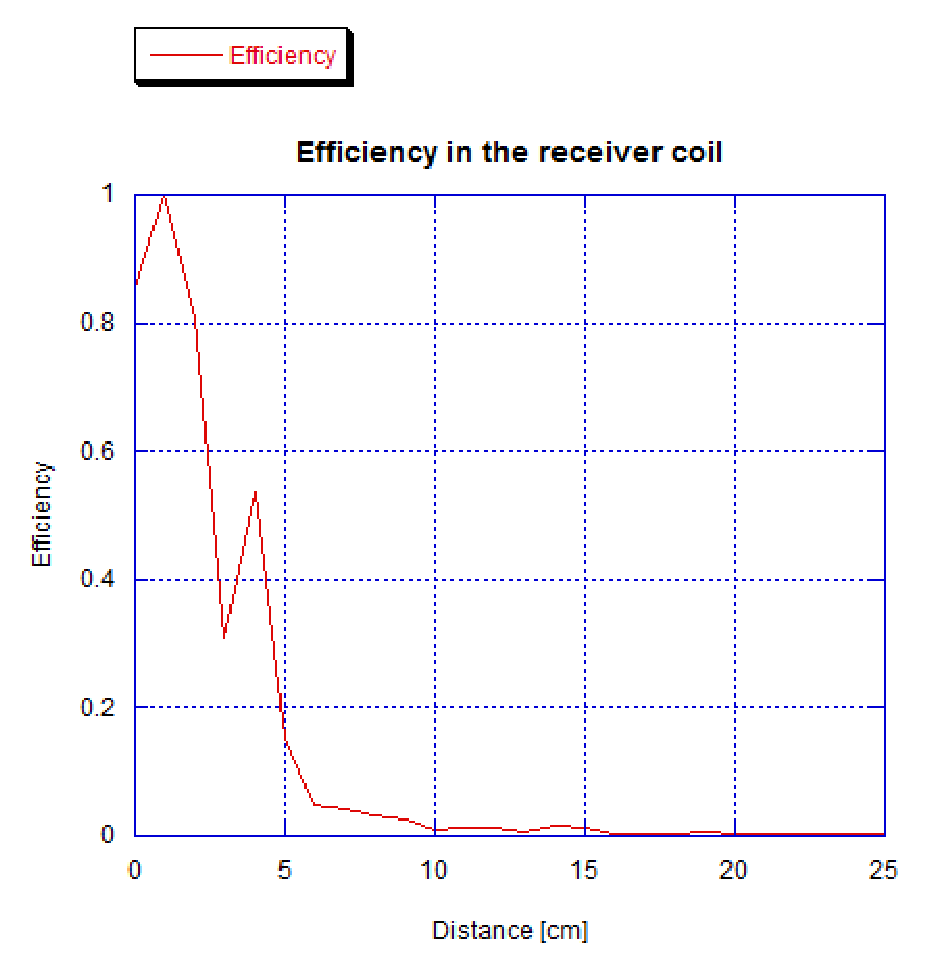
\includegraphics{11_efficiency_circular.eps}}&
\scalebox{0.35}[0.4]{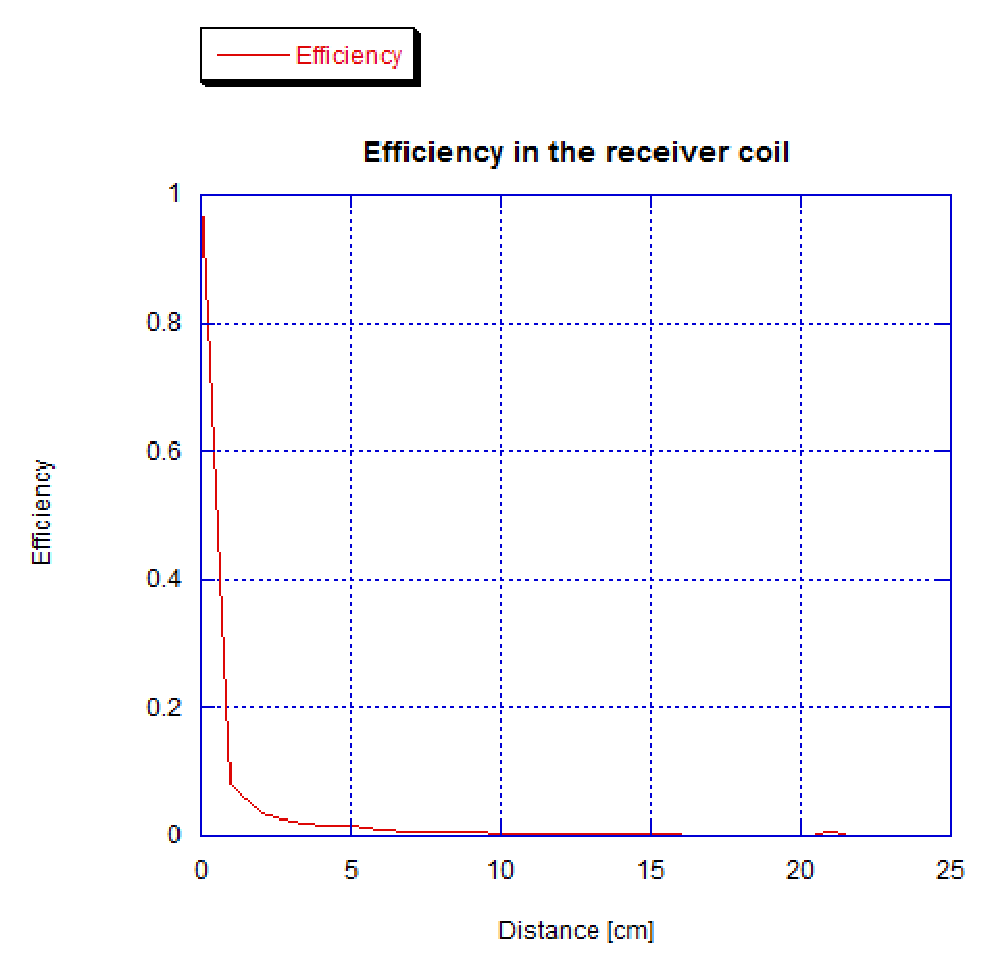
\includegraphics{12_efficiency_triangular.eps}}\\
a)&b)\\
\end{tabular}
} \caption{Normalized efficiency for (a) circular and (b) triangular coils.}\label{fig:exp_6}
\end{center}
\end{figure}

Finally, the graphical form of the spatial distribution of the energy was measured. The radiation pattern for circular and triangular coils is shown in figure \ref{fig:exp_7}. It's interesting to observe that, in low frequency the radiation pattern is uniform and it has 2 lobes and they are centered on the axis X. In medium frequencies, the radiation patter is deformed and it has 4 lobes which are not centered on the axis X.

\begin{figure}[tbp]
\begin{center}
\fbox{
\begin{tabular}{cc}
\scalebox{0.35}[0.4]{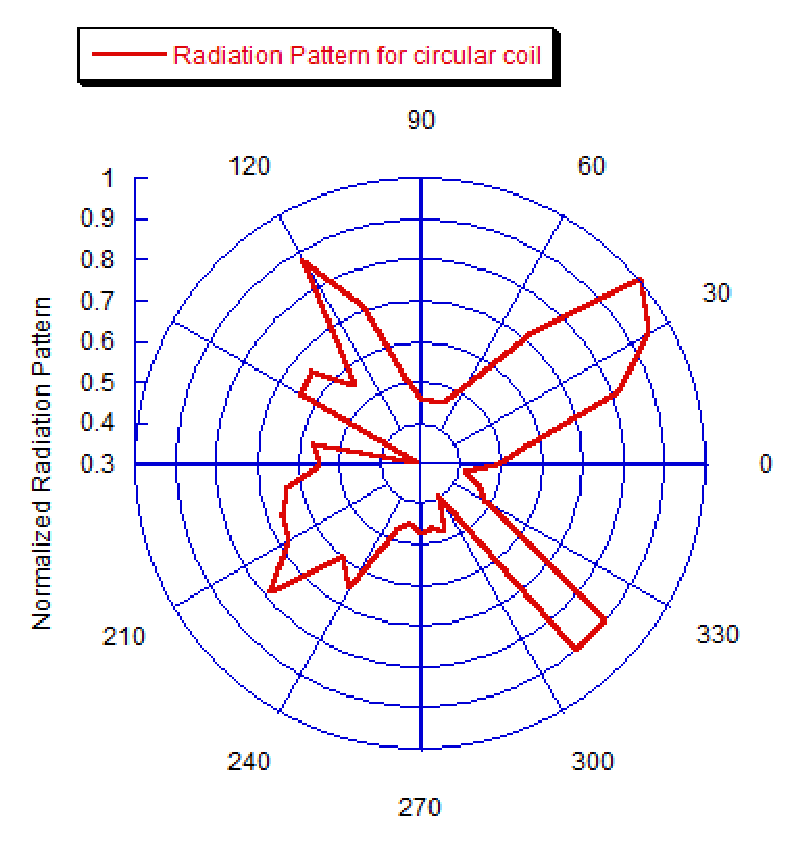
\includegraphics{13_PR_circular.eps}}&
\scalebox{0.35}[0.4]{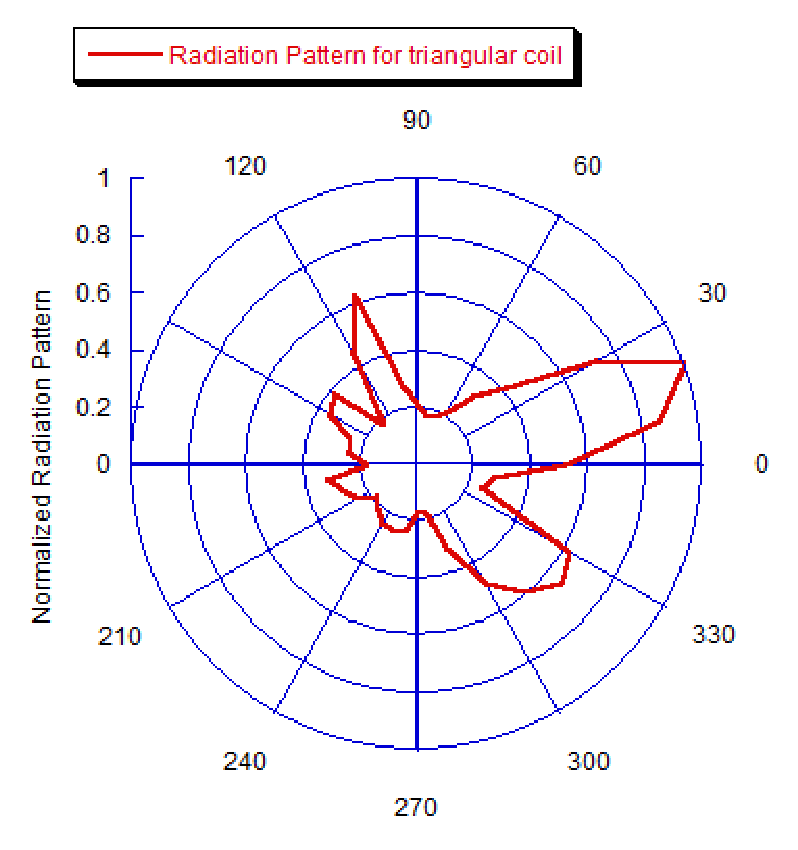
\includegraphics{14_PR_triangular.eps}}\\
a)&b)\\
\end{tabular}
} \caption{Radiation pattern for (a) circular and (b) triangular coils.}\label{fig:exp_7}
\end{center}
\end{figure}






\end{document}
